\documentclass[12pt]{article}
\usepackage[czech]{babel}
\usepackage[utf8]{inputenc}
\usepackage[plainpages=false,pdfpagelabels,unicode]{hyperref}
\usepackage[pdftex]{graphicx}
\usepackage[margin=2cm, includefoot]{geometry}

\begin{document}

\title{Experimentální metody a speciální praktikum \\
Studium činnosti ICCD detektoru}
\author{Pavel Ondračka, Roman Petráš a Vojtěch Homola}
\maketitle

\section{Úvod}
ICCD detektor sa využíva k záznamu spektrálnej závislosti intenzity vyžarovania, prednostne periodických signálov a zdrojov nízkej intenzity.
Fotón dopadajúci na katódu emituje elektrón. K zosilneniu signálu sa používa mikrokanálová doštička, ktorá spĺňa úlohu fotonásobiča. Znásobené elektróny sú následne urýchľované smerom k vrstvičke luminofóru, čím dochádza k emisii fotónov, ktoré sú vedené optickým káblom na CCD snímač (obrázek \ref{}).
Počas experimentu sme používali spektrometer Horiba Jobin Zvon 1024x256-18UVF s ICCD detektorom. ICCD detektor byl během měření chlazený jednoduchým peltierovým článkem na -10\,$^\circ$C.
Merala sa časová závislosť intenzity vyžarovania LED diódy (vlnová dĺžka 633nm, krátka nábežná dráha cca 25ns) budenej obdĺžnikovými pulzmi. Dióda sa budila generátorom obdĺžnikových pulzov, ktorý také slúžil ako externý trigger pre spektrometer pracujúci v režime slave.
Parametre, ktoré sa pri meraní menili boli: frekvencia zdroja obdĺžnikových pulzov $f$, delay $t$ -- čas synchronizácie , krok delay $t_d$, délka pulzu $\Delta t$ – časové rozlíšenie výstupnej závislosti, a integračná doba $\tau$, čo je doba počas ktorej sa signál zbiera pre hodnotu intenzity v rámci jedného pulzu.
Detektor funguje tak, že v čase t=0 triggerovacej periódy začne s triggerovaciou frekvenciou spínať ICCD a hromadiť signál vždy v čase t=0 triggerovacej cez integračnú dobu. Následne prechádza na čas $t = t + t_d$  a vykoná to isté. Proces sa opakuje počas celého rozsahu doby meškania t. dostávame graf závislosti intenzity žiarenia na čase definičného oboru danom časom synchronizácie.


\begin{figure}[htbp]
\begin{center}
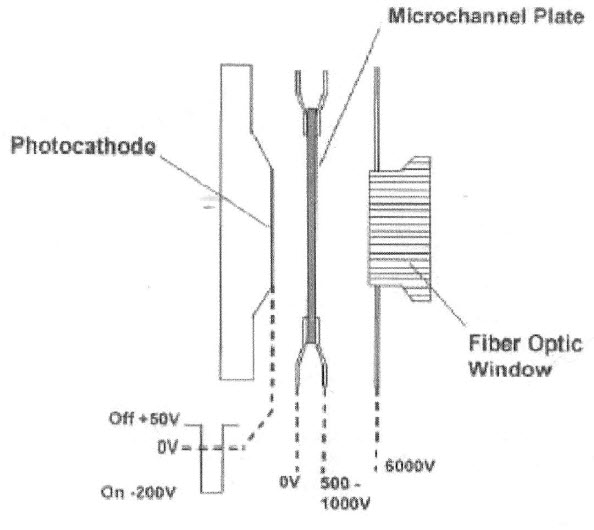
\includegraphics[width=8cm]{img1.png}
\caption{Schéma zesilovače používaného v ICCD}
\label{}
\end{center}
\end{figure}

\section{Měření}
Na začátku bylo provedeno měření obyčejným CCD detektorem pro kontrolu (obrázek \ref{ccd}). Naměřené spektrum odpovídá očekávanému spektru diody, malý artefakt na cca 610\,nm je světlo z rtuťové výbojky. ICCD kamera také umí měřit na různých vlnových délkách, ale my jsme se při měření omezili pouze na jednu vlnovou délku a zkoumali jsem časový průběh signálu.


\begin{figure}[htbp]
\begin{center}
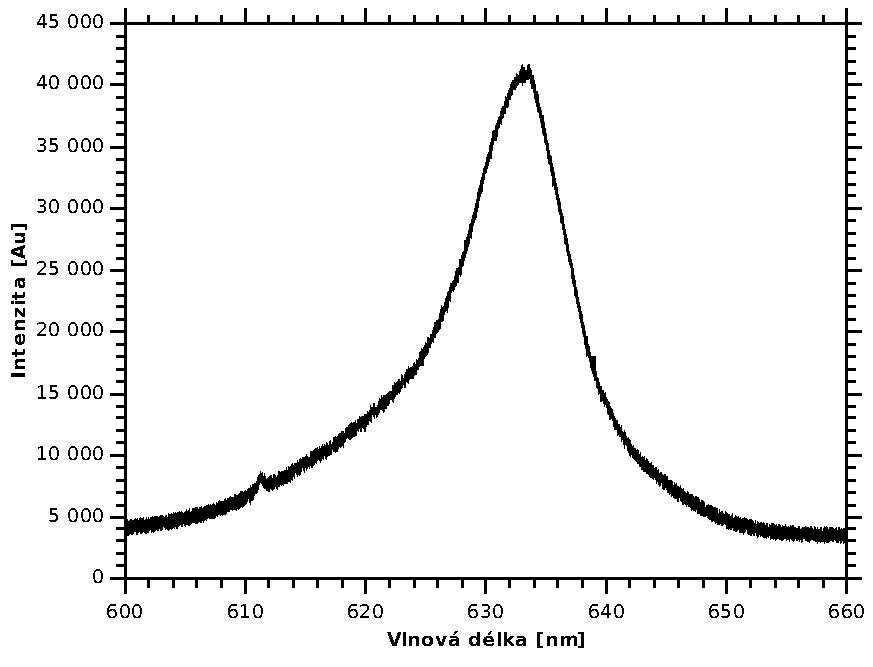
\includegraphics[width=12cm]{ccddioda.pdf}
\caption{Část spektra diody měřené na běžném CCD detektoru}
\label{ccd}
\end{center}
\end{figure}

Jako první zkoumáme závislost intenzity signálu na integrační době (obrázek \ref{intdoba}). Zde se podle předpokladu s dvojnásobnou integrační dobou zdvojnásobí i intenzita signálu, také se ale zdvojnásobí intenzita pozadí a celková doba měření. Pokles intenzity v druhé periodě je způsoben tím, že kvůli velkému delay se detektor aktivuje jen každou druhou periodu, z toho důvodu je tedy signál poloviční.

\begin{figure}[htbp]
\begin{center}
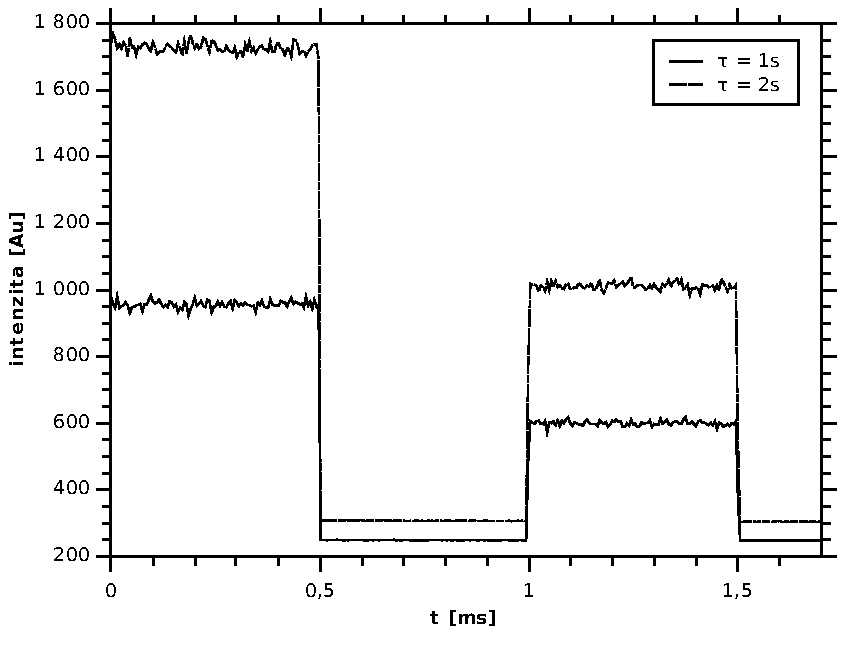
\includegraphics[width=12cm]{intdoba.pdf}
\caption{Závislost intenzity signálu na integrační době, gain = 50, $f$ = 1\,kHz, $t_d$ = 5\,$\mu$s,\newline $\Delta t$ = 5\,$\mu$s}
\label{intdoba}
\end{center}
\end{figure}

Dalším způsob jak získat silnější signál je větší zesílení (gain), průběh signálu pro dvě hodnoty gainu je na obrázku \ref{gain2}. Zesílení gainu nemá vliv na intenzitu pozadí, protože ta vzniká až za násobičem (tepelným šumem na detektoru). Nicméně příliš velkým zesílení je možno násobič elektronů poškodit. 

\begin{figure}[htbp]
\begin{center}
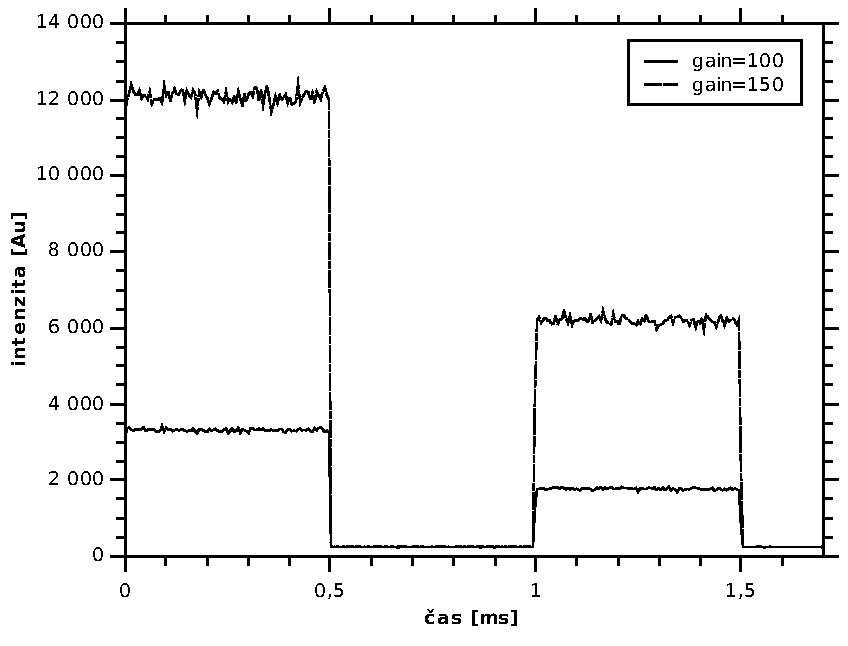
\includegraphics[width=12cm]{gain2.pdf}
\caption{Závislost intenzity signálu na gainu, $f$ = 1\,kHz, $t_d$ = 5\,$\mu$s, $\Delta t$ = 5\,$\mu$s, $\tau$ = 1s}
\label{gain2}
\end{center}
\end{figure}

Další z parametrů který lze při měření měnit je délka pulzu, při předchozích měřeních byla 5\,$\mu$s. Na obrázku \ref{delka} je měření při kterém byla délka pulzu zvětšena 10$\times$ na 50\,$\mu$s. K nárůstu signálu sice nedošlo, ale to je způsobeno tím, že byl současně snížen gain na 50 a integrační doba na 0,5\,s. Pokud bychom nechali ostatní parametry na předchozích hodnotách, získaly bychom 10$\times$ silnější signál. Nevýhodou je zprůměrování signálu za delší dobu, které se projevuje vyhlazením signálu křivky a zkosením náběhové hrany.

\begin{figure}[htbp]
\begin{center}
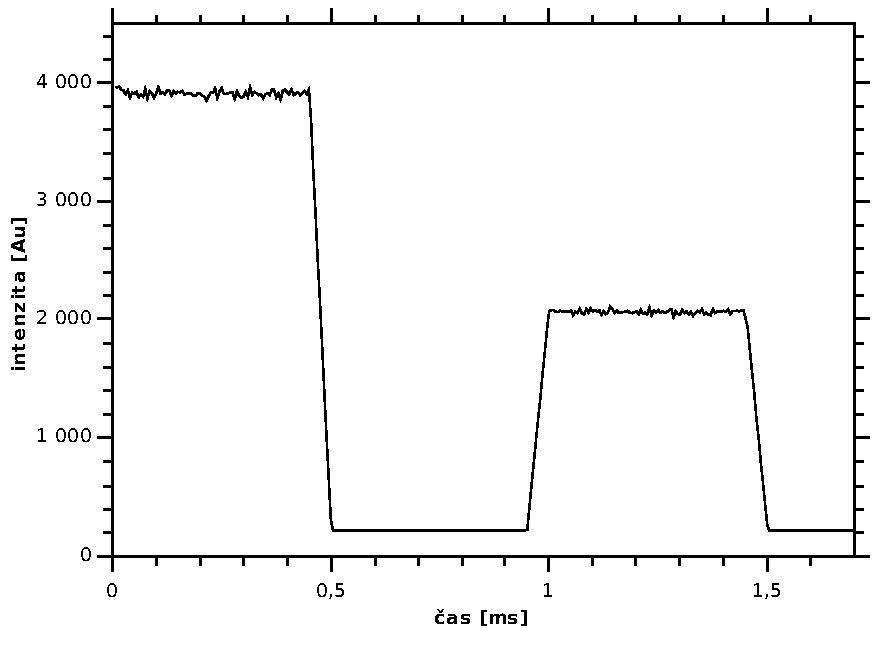
\includegraphics[width=12cm]{delka.pdf}
\caption{Průběh signálu při změně délky pulzu, gain=50, $f$ = 1\,kHz, $t_d$ = 5\,$\mu$s, $\Delta t$ = 50\,$\mu$s,\newline $\tau$ = 0,5s}
\label{delka}
\end{center}
\end{figure}

Poslední parametr který můžeme během měření měnit je krok delay $t_d$, ten má vliv na celkový počet naměřených bodů. Jak vypadá průběh signálu pro 10$\times$ zvětšený krok delay je na obrázku \ref{delka}.

\begin{figure}[htbp]
\begin{center}
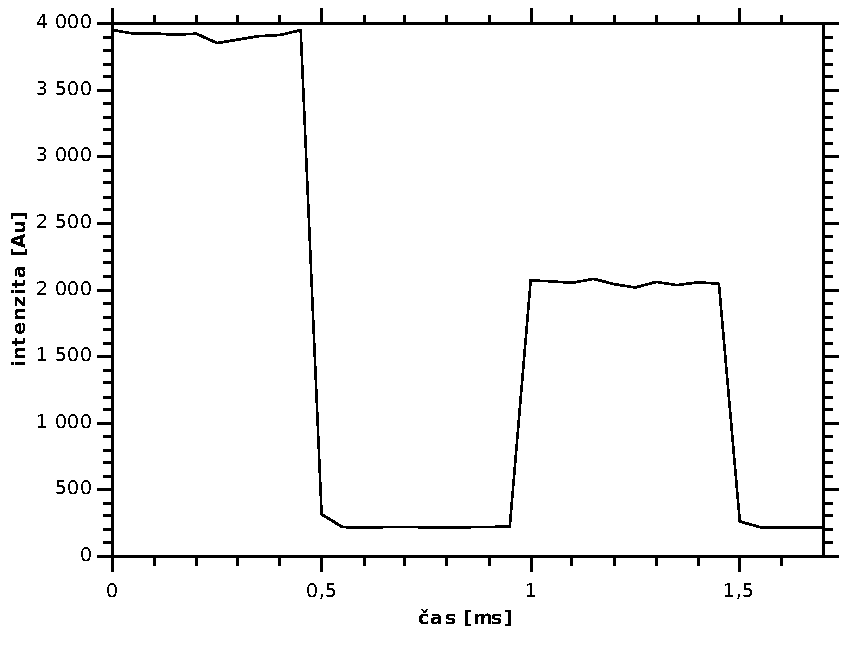
\includegraphics[width=12cm]{krokdelay.pdf}
\caption{Průběh signálu při změně kroku delay, gain=50, $f$ = 1\,kHz, $t_d$ = 50\,$\mu$s, $\Delta t$ = 50\,$\mu$s,\newline $\tau$ = 0,5s}
\label{krokdelay}
\end{center}
\end{figure}

Nakonec byla změněna frekvence diody na 10\,kHz a vyzkoušeli jsme si odhad parametrů abychom dostali dobrý signál. Na obrázku \ref{gain2} je závislost intenzit pulzů diody pro různé hodnoty gainu. Na obrázku \ref{gain5} je zprůměrovaná hodnota intenzity za čas 50\,$\mu$s (doba zapnutí diody v jedné periodě), je zde vidět že intenzita signálu se zvyšováním gainu nestoupá lineárně.

\begin{figure}[htbp]
\begin{center}
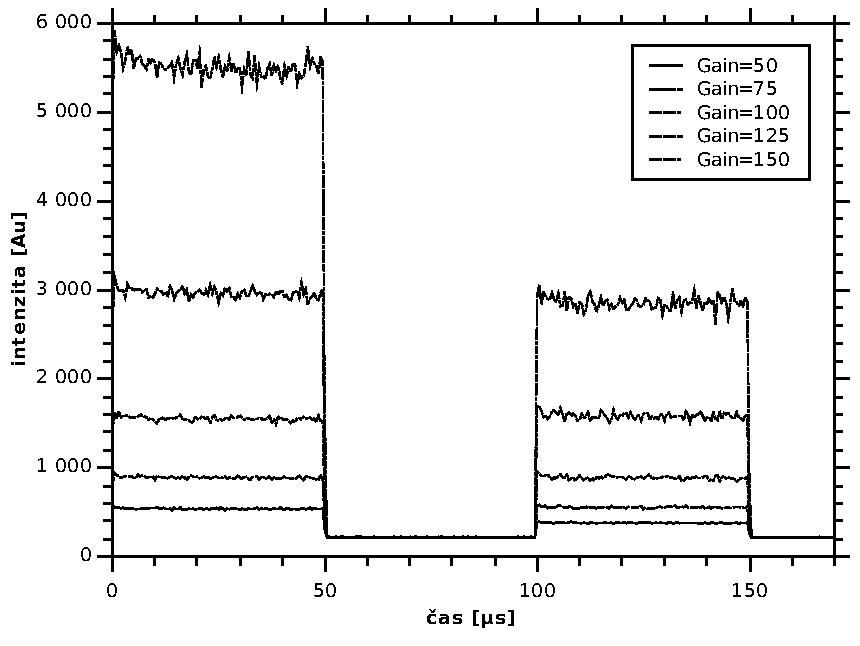
\includegraphics[width=12cm]{intensityformoregains.pdf}
\caption{Časový průběh intenzity signálu pro různé hodnoty gainu, $f$ = 10\,kHz, $t_d$ = 0,5\,$\mu$s, $\Delta t$ = 0,5\,$\mu$s, $\tau$ = 0,5\,s}
\label{gain3}
\end{center}
\end{figure}

\begin{figure}[htbp]
\begin{center}
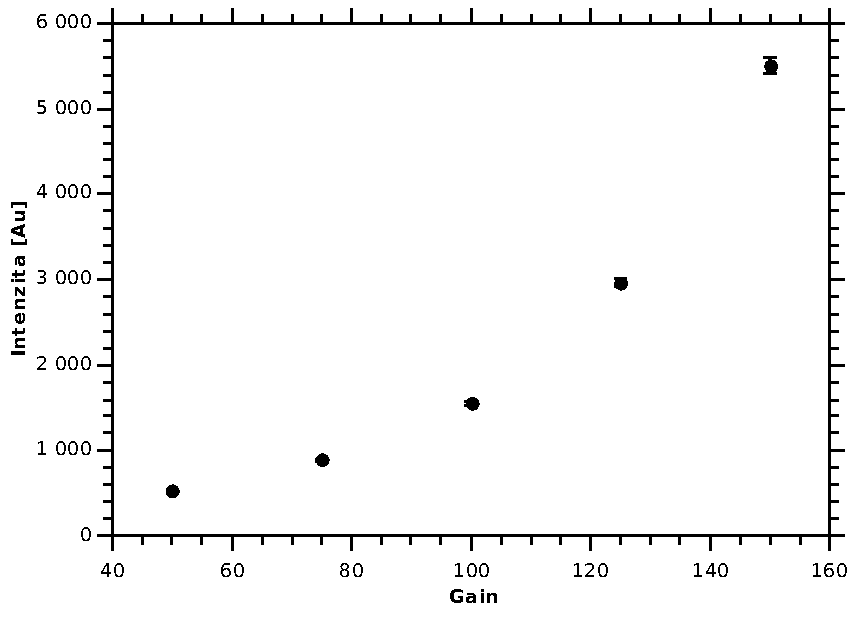
\includegraphics[width=12cm]{intensityongain.pdf}
\caption{Závislost průměrné intenzity signálu na zesílení (gain)}
\label{gain5}
\end{center}
\end{figure}

\newpage

\section{Závěr}
Praktikum proběhlo úspěšně. Podařilo se vyzkoušet činnost ICCD detektoru a vliv jednotlivývh parametrů měření na výsledný signál. Ukázalo se, že volba parametrů je vždy kompromis mezi kvalitou a délkou měření. Špatná volba jednotlivých parametrů může vézt ke zkreslení signálu například pokud zvolíme délku pulzu delší nebo srovnatelnou s periodou signálu. Také si musíme dávat pozor na velikost gainu, abychom nepoškodili násobič elektronů. Přes nevýhody ve složitějším principu a nastavení se ICCD kamera ukázala jako vhodný nástroj pro měření krátkých periodických pulzů, které bychom běžnou CCD kamerou vůbec nezaznamenali. 

\end{document}
